\documentclass[12pt,letterpaper]{hmcpset}
\usepackage[margin=1in]{geometry}
\usepackage{graphicx}
\usepackage{amsmath,amssymb}
\usepackage{enumerate}

% info for header block in upper right hand corner
\name{}
\class{Physics 24a - Section ---}
\assignment{assignment}
\duedate{date}

\begin{document}

\problemlist{7.\{4,8,9,13,22\}}

\textbf{Reading:} Chapter 7

\begin{problem}[1 - Grazing instrument package - KK 7.4]
    A spaceship is sent to investigate a planet of
    mass $M$ and radius $R$. While hanging motionless
    in space at a distance $5R$ from the center of
    the planet, the ship fires an instrument package
    with speed $v_{0}$, as shown in the sketch. The
    package has mass $m$, which is much smaller than
    the mass of the spaceship. For what angle $\theta$
    will the package just graze the surface of the planet?

    \begin{center}
    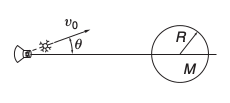
\includegraphics[width=2in]{img/7_4}
    \end{center}
\end{problem}

\begin{solution}
    \vfill
\end{solution}
\clearpage

\begin{problem}[2 - Moment of inertia of a sphere* - KK 7.8]
    Find the moment of inertia of a uniform 
    sphere of mass $M$ and radius $R$ about
    an axis through the center.
\end{problem}

\begin{solution}
    \vfill
\end{solution}
\clearpage

\begin{problem}[3 - Bar and rollers - KK 7.9]
    A heavy uniform bar of mass $M$ rests on top 
    of two identical rollers that are continuously
    turned rapidly in opposite directions, as shown. 
    The centers of the rollers are a distance $2l$
    apart. The coefficient of friction between the
    bar and roller surfaces is $\mu$, a constant
    independent of the relative speed of the two
    surfaces. Initially the bar is held at rest with
    its center at distance $x_{0}$ from the midpoint
    of the rollers. At time $t = 0$ it is released. 
    Find the subsequent motion of the bar. 
    (Assume that the bar is thin.)
    \begin{center}
        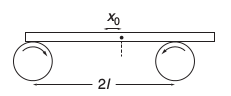
\includegraphics[width=2in]{img/7_9}
    \end{center}
\end{problem}

\begin{solution}
    \vfill
\end{solution}
\clearpage

\begin{problem}[4 - Mass and post - KK 7.13]
    A mass $m$ is attached to a post of radius $R$
    by a string. Initially it is distance $r$ from
    the center of the post and is moving tangentially
    with speed $v_{0}$.

    \emph{Case (a)} The string passes through a hole 
    in the center of the post at the top. The string
    is gradually shortened by drawing it through the hole.

    \emph{Case (b)} The string wraps around the outside
    of the post. 
 
    What quantities are conserved in each case? Find 
    the final speed of the mass when it hits the post
    for each case.

    \begin{center}
        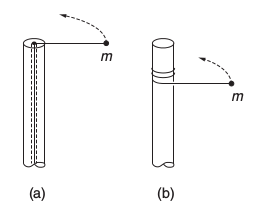
\includegraphics[width=2in]{img/7_13}
    \end{center}
\end{problem}

\begin{solution}
    \vfill
\end{solution}
\clearpage

\begin{problem}[5 - Bead and rod - KK 7.22]
    A bead of mass $m$ slides without friction
    on a rod that is made to rotate at a constant
    angular speed $\omega$. Neglect gravity.
    \begin{enumerate}[(a)]
    \item Show that $r = r_{0} e^{\omega t}$ is a 
        possible motion of the bead, where $r_{0}$ 
        is the initial distance of the bead from the 
        pivot.
    \item For the motion described in part (a), find 
        the force exerted by the bead on the rod.
    \item For the motion described above, find the 
        power exerted by the agency that is turning 
        the rod and show by direct calculation that
        this power equals the rate of change of kinetic
        energy of the bead.
    \end{enumerate}

    \begin{center}
        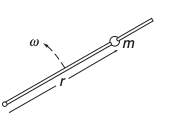
\includegraphics[width=1.5in]{img/7_22}
    \end{center}
\end{problem}

\begin{solution}
    \vfill
\end{solution}
\clearpage

\end{document}
